\section{Experimental Results}
\label{sec:result}

We simulate the behavior of the proposed lattice PUF in Python. The statistical model of raw SRAM POKs is based on \cite{maes2013accurate, maes2009soft}. The logical behavior of other digital circuits are accurately captured by software. We virtually manufacture (simulate) $1000$ distinct lattice PUF instances with design parameters chosen in Section \ref{sec:design}. Their CRPs are collected to evaluate: (1) statistical properties (uniformity, uniqueness, and reliability), and (2) resistance to state-of-the-art ML attacks. The entire lattice PUF system (except for the raw SRAM cells) is implemented on a Spartan 6 FPGA.


\subsection{Statistical Analysis}
\label{sec:statistical_result}
\textbf{Uniformity} of a PUF characterizes unbiasedness, namely, the proportion of `0's and `1's in the output responses.
For an ideal PUF $f$, the proportion needs to be $50\%$ for either `0' or `1'.
Uniformity is formally defined as the average Hamming weight $\HW(f)$ of responses $\mathbf{r}$ over randomly sampled challenges $\mathbf{c}$'s \cite{maiti2013systematic}:
\begin{equation*}
\HW(f)= \Expect_\mathbf{c}[\HW(\mathbf{r})] = \Expect_{\mathbf{c}}[\HW(f(\mathbf{c}))].
\end{equation*}
Here $\Expect_X$ represents expectation over random variable $X$.
Note that $\mathbf{c}$ follows the ciphertext distribution rather than the usual uniform distribution \cite{maiti2013systematic}.
Figure \ref{fig:HW} shows uniformity obtained using $1000$ randomly selected challenges. 
The distribution is centered at $49.98\%$, the standard deviation is $1.58\%$. 


\textbf{Uniqueness} measures the ability of a PUF to be uniquely distinguished among a set of PUFs. 
Based on \cite{maiti2013systematic}, we define this metric to be the average inter-class HD of responses $(\mathbf{r}_i,\mathbf{r}_j)$ under the same challenges $\mathbf{c}$ for a randomly picked PUF pair $(f_i, f_j)$:
\begin{equation*}
\HD(f_i,f_j) = \Expect_\mathbf{c}[\HD(\mathbf{r}_i,\mathbf{r}_j)]=\Expect_{\mathbf{c}}[\HD(f_i(\mathbf{c}),f_j(\mathbf{c}))].
\end{equation*}
For ideal PUFs, responses under the same challenges are orthogonal, namely, $\HD(f_i,f_j)$'s are close to $50\%$.
Uniqueness is also evaluated under the ciphertext distribution.  

Uniqueness is shown in Figure \ref{fig:inter_intra}, evaluated for $1000$ PUF instances. 
The lattice PUF achieves near-optimal uniqueness: inter-class HD is centered at $50.00\%$, its standard deviation is $1.58\%$. 

\textbf{Reliability} of a PUF $f$ is characterized by the average BER of outputs with respect to their enrollment values:
\begin{equation*}
\BER = \Expect_{f^\prime}[\HD(f,f^\prime)]= \Expect_{f^\prime,\mathbf{c}}[\HD(f(\mathbf{c}),f^\prime(\mathbf{c}))].
\end{equation*}
As discussed in Section \ref{sec:design}, the overall BER of the lattice PUF is due to two components: the failure rate of key reconstruction and LWE decryption error rate.
Intra-class HD in Figure \ref{fig:inter_intra} reflects the result of decryption errors by assuming a perfect key reconstruction. 

%\begin{figure}[t!]
%\centering
%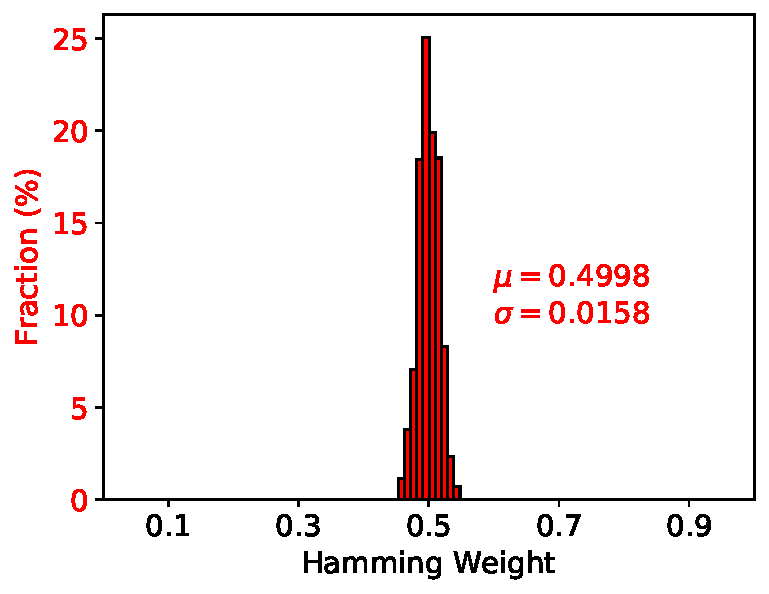
\includegraphics[width = 0.7\linewidth]{./figs/HW.pdf}
%\caption{Uniformity of lattice PUF output.}
%\label{fig:HW}
%\end{figure}

%\begin{figure}[t!]
%\centering
%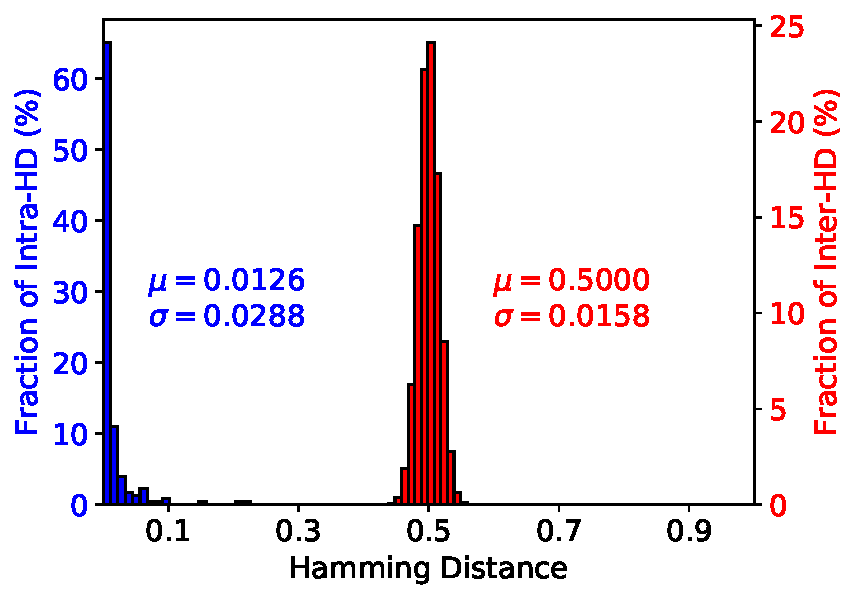
\includegraphics[width = 0.75\linewidth]{./figs/inter_intra.pdf}
%\caption{Uniqueness and reliability of lattice PUF output.}
%\label{fig:inter_intra}
%\end{figure}

\begin{figure} 
    \centering
  \subfloat[\label{fig:HW}]{%
       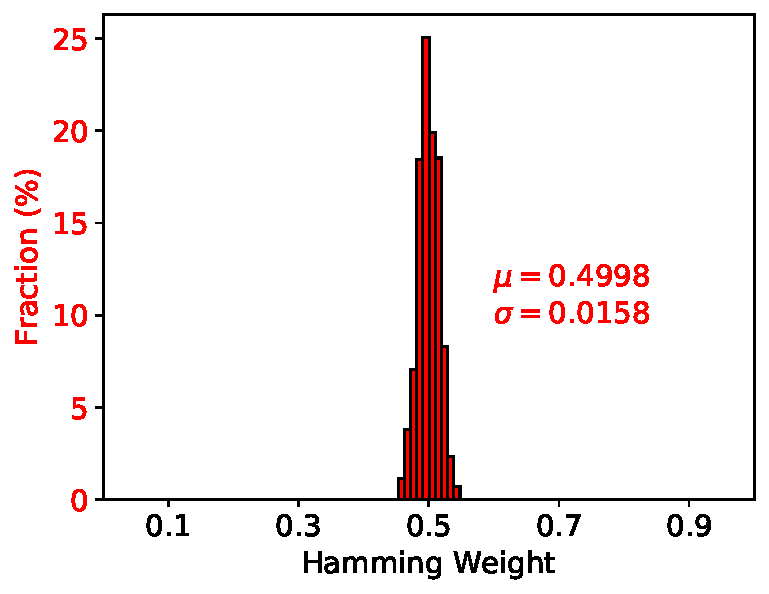
\includegraphics[width=0.45\linewidth]{./figs/HW.pdf}}
    \hfill
  \subfloat[\label{fig:inter_intra}]{%
        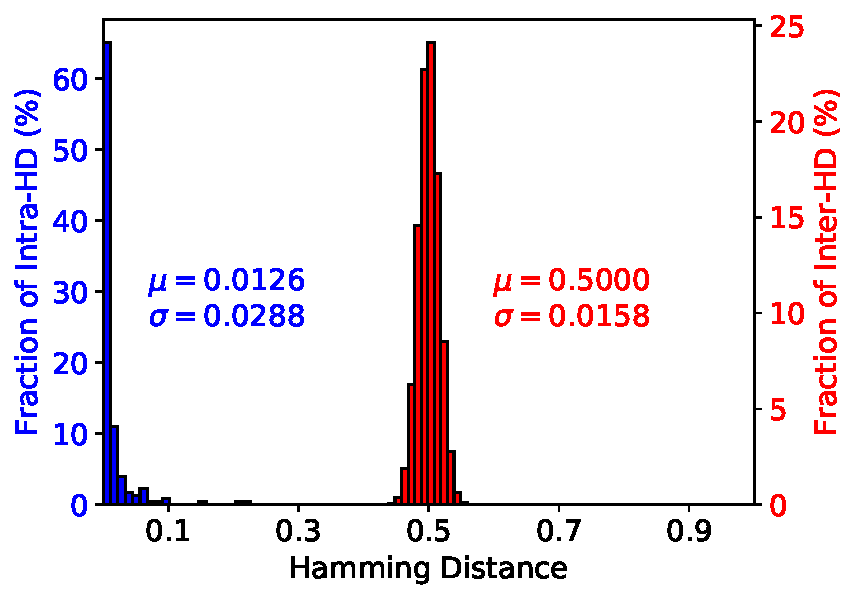
\includegraphics[width=0.5\linewidth]{./figs/inter_intra.pdf}}
  \caption{(a) Uniformity of lattice PUF output. (b) Uniqueness and reliability of lattice PUF output.}
  \label{fig: lattice_puf_stats} 
\end{figure}

%\begin{figure}[t!]
%\centering
%\begin{subfigure}{0.2\textwidth}
%   \centering
%   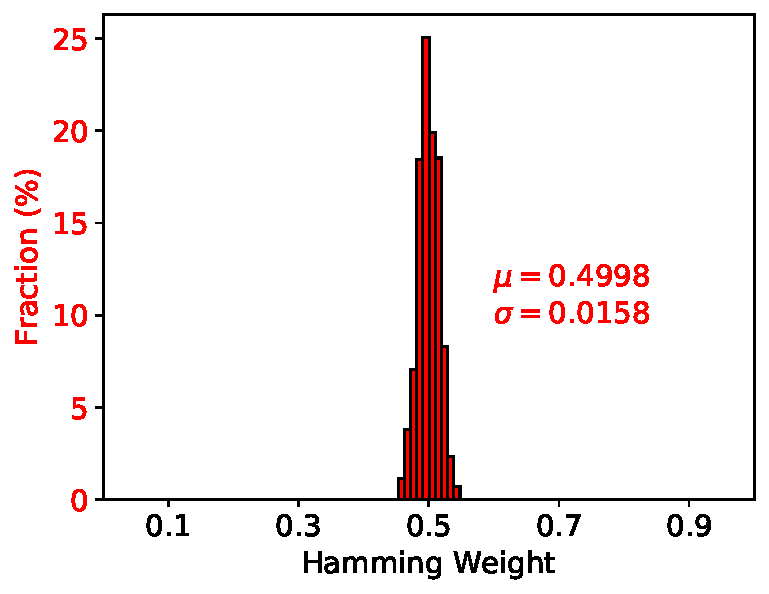
\includegraphics[width=\textwidth]{./figs/HW.pdf}
   %\caption{Uniformity of lattice PUF output.}
%   \label{fig:HW} 
%\end{subfigure}
%\begin{subfigure}{0.24\textwidth}
%   \centering
%   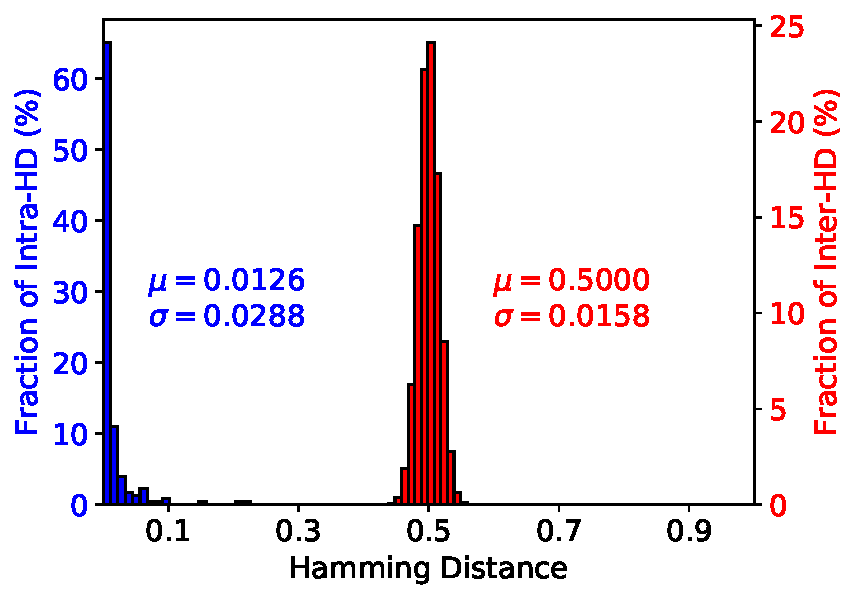
\includegraphics[width=\textwidth]{./figs/inter_intra.pdf}
   %\caption{Uniqueness and reliability of lattice PUF output.}
%   \label{fig:inter_intra}
%\end{subfigure}
%\caption{(a) Uniformity of lattice PUF output. (b) Uniqueness and reliability of lattice PUF output.}
%\label{power_trace_avg_untrusted_devices_1_to_15}
%\end{figure}

\subsection{Empirical ML Resistance}

While the ultimate promise of lattice PUF is due to its theoretically-supported reliance on hard computational problems,
testing its ML resistance empirically gives a concrete measure of its security. The resistance of lattice PUF is evaluated with a series of traditional (i.e., not based on deep learning) ML algorithms, including SVM, LR, and single-layer NN (1-NN), as well as a number of DNNs.
We use the Python scikit-learn %\cite{scikit-learn} 
package to implement SVM and LR.  
The SVM uses the radial basis function (RBF) kernel.
The 1-NN model uses only one hidden feed-forward layer composed of 100 neurons, with the rectified linear unit (ReLU) as the activation function. 
Training of 1-NNs and subsequent DNNs are implemented using Keras %\cite{chollet2015keras} 
with TensorFlow %\cite{abadi2016tensorflow} 
backend. 

\begin{figure}[t!]
\centering
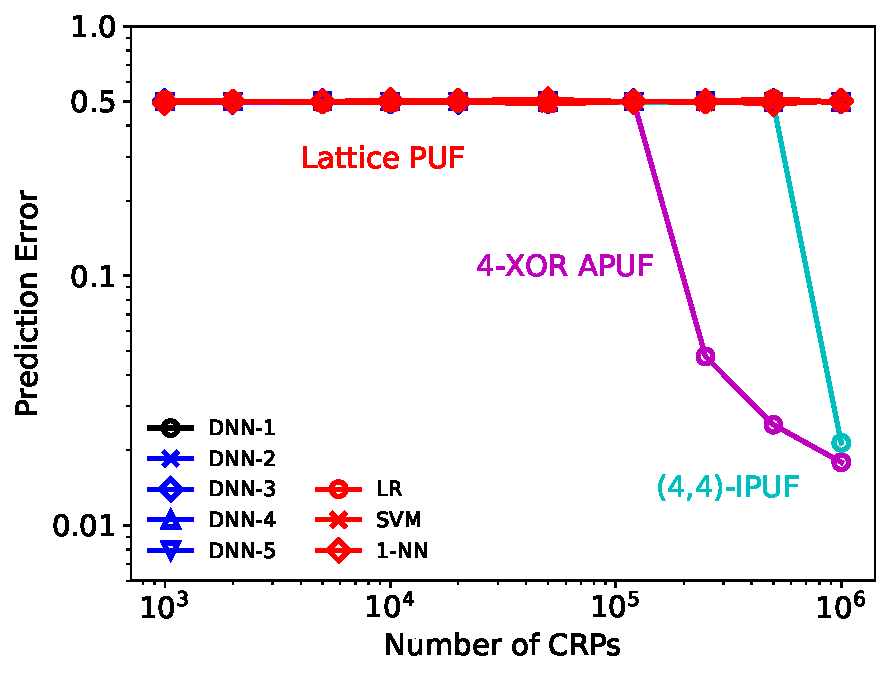
\includegraphics[width = 0.7\linewidth]{./figs/ml_attack_dnn_all_puf_5.pdf}
\caption{ML attacks: Lattice PUF remains resistant to all attacks (DNNs, LR, SVM,1-NN). DNN ultimately succeeds in modeling two other strong PUFs.}
\label{fig:ml_attack_2}
\end{figure}

\begin{figure}[t!]
\centering
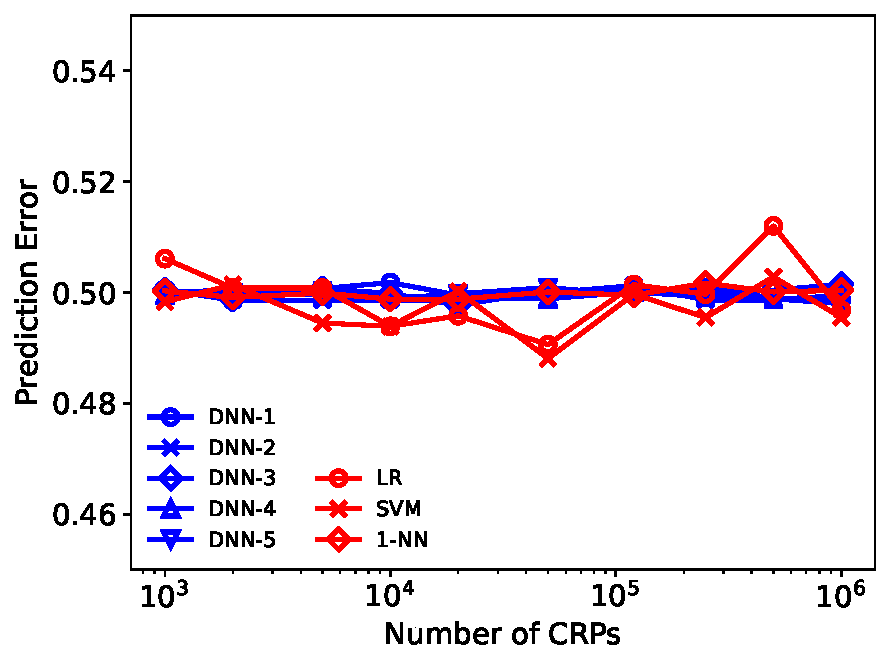
\includegraphics[width = 0.7\linewidth]{./figs/ml_attack_lattice_puf.pdf}
\caption{Lattice PUF is resistant to both traditional ML attacks and DNNs.}
\label{fig:ml_attack_3}
\end{figure}

%\begin{figure}[t!] 
%    \centering
%  \subfloat[\label{fig:ml_attack_2}]{%
%       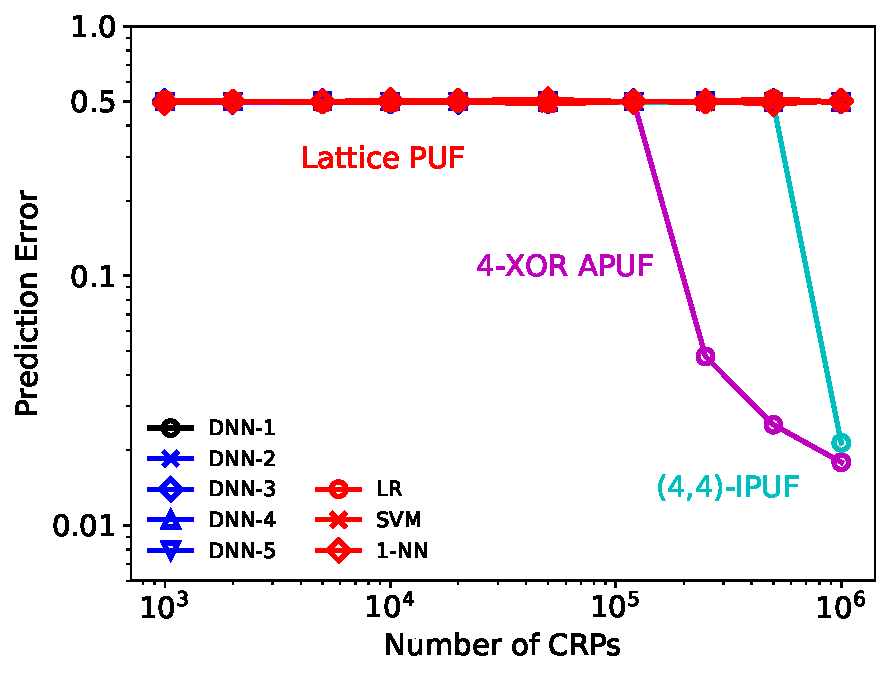
\includegraphics[width=0.5\linewidth]{./figs/ml_attack_dnn_all_puf_5.pdf}}
%    \hfill
%  \subfloat[\label{fig:ml_attack_3}]{%
%        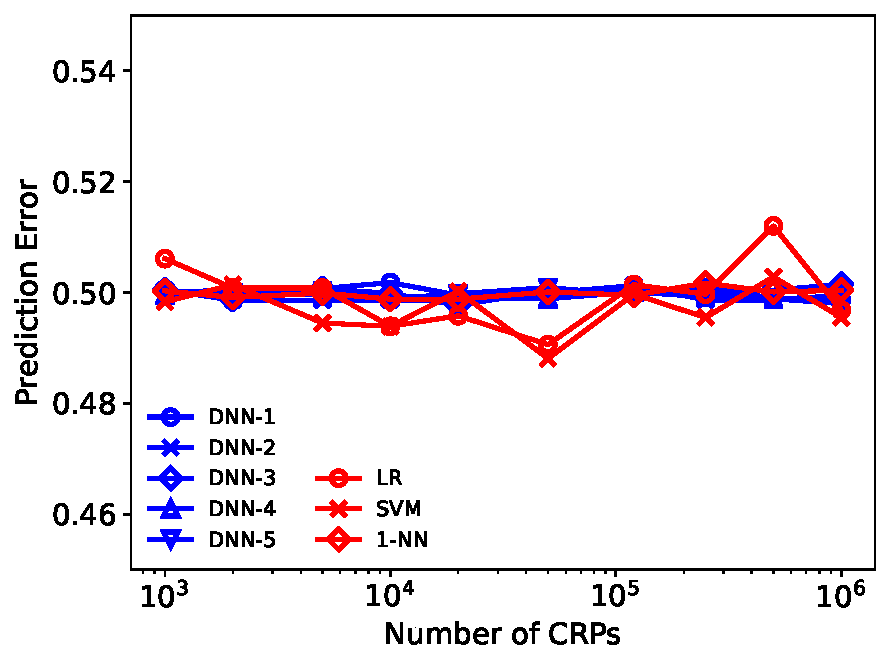
\includegraphics[width=0.5\linewidth]{./figs/ml_attack_lattice_puf.pdf}}
%  \caption{(a) ML attacks: Lattice PUF remains resistant to all attacks (DNNs, LR, SVM,1-NN). DNN ultimately succeeds in modeling two other strong PUFs. (b) Lattice PUF is resistant to both traditional ML attacks and DNNs.}
%  \label{fig: lattice_puf_ml_attack_results} 
%\end{figure}

\begin{table}[t!]
\centering
	\caption{Various configuration for DNN attacks.}
	\label{table:DNNSetting}
	\resizebox{\linewidth}{!}{
        \begin{tabular}{|l|l|l|l|l|l|}
        \hline
        \textbf{Setup} & \begin{tabular}[c]{@{}l@{}}\textbf{Hidden}\\ \textbf{Layers}\end{tabular} & \begin{tabular}[c]{@{}l@{}}\textbf{Neurons}\\ \textbf{per Layer}\end{tabular} & \begin{tabular}[c]{@{}l@{}}\textbf{Challenge} \\ \textbf{Distribution}\end{tabular} & \begin{tabular}[c]{@{}l@{}}\textbf{Input} \\ \textbf{Format}\end{tabular} & \begin{tabular}[c]{@{}l@{}}\textbf{Prediction}\\ \textbf{Error}\end{tabular} \\ \hline
        DNN-1     & 4                                                       & 100                                                         & PRNG                                                              & Binary                                                  & 49.86\%                                                       \\ \hline
        DNN-2     & 4                                                       & 100                                                         & PRNG                                                              & Real                                                    & 49.84\%                                                       \\ \hline
        DNN-3     & 4                                                       & 100                                                         & Ciphertext                                                        & Binary                                                  & 49.76\%                                                       \\ \hline
        DNN-4     & 6                                                       & 100                                                         & PRNG                                                              & Binary                                                  & 49.80\%                                                       \\ \hline
        DNN-5     & 4                                                       & 200                                                         & PRNG                                                              & Binary                                                  & 49.87\%                                                       \\ \hline
        \end{tabular}
    }
\end{table}

DNNs are more powerful in binary classification. DNNs contain multiple hidden layers which enable superior modeling expressiveness compared to 1-NNs \cite{goodfellow2016deep}. Notably, recent successful DNN-based attacks have been demonstrated on published strong PUFs, including XOR APUFs and IPUFs \cite{DBLP:journals/iacr/SantikellurBC19}. Our baseline DNN experiment (DNN-1) adopts the same network parameters as in \cite{DBLP:journals/iacr/SantikellurBC19}.  The network has 4 hidden layers, each containing 100 neurons. It uses ReLU as the non-linear operator. 

Besides the parameters used in the baseline experiment, we varied network architectures, hyper-parameters, and numeric representations in the attack, as listed in Table \ref{table:DNNSetting}. 
DNN-2 treats input as 161 integer numbers from 0 to 255, instead of 1288 binary bits.
DNN-3 is different from the baseline version in its CRP generation strategy (see more below).
DNN-4 and DNN-5 add more hidden layers and more neurons per hidden layer respectively, compared to the baseline DNN-1.

Figure \ref{fig:ml_attack_2} shows the results of the empirical attacks based on the above ML algorithms. The figure shows the prediction error of lattice PUF in response to these attacks with training set size ranging from $1000$ to $1$ million and test set of size $200$K. The Adam optimizer \cite{kingma2014adam} terminates after 200 epochs, and results in a prediction error of $49.86\%$, barely better than a random guess. \emph{The results show that the prediction error of lattice PUF remains flat for all attempted attacks: across the range of attacks and CRP training set sizes, there is no measurable deviation of the error from 0.5.} In contrast, a DNN (with a configuration corresponding to DNN-1) achieves less than $2\%$ prediction error for both 4-XOR APUF and (4, 4)-IPUF. 

It is important to note that the experiments also show that the use of distributional relaxation of space-efficient LWE (described in Section \ref{sec:lfsr}) does not hinder empirical ML resistance of lattice PUF. In Table 1, all design/attack combinations except for DNN-3 are based on the compact (relaxation-based) design in which CRPs are generated via a PRNG. Finally, we show a detailed view of ML attack results on lattice PUF in Figure \ref{fig:ml_attack_3} by zooming in Figure \ref{fig:ml_attack_2}. While run-to-run variations of the training optimizer are observable, the prediction error remains close to $50\%$.

\subsection{Hardware Implementation Results}
\label{sec:hardware_results}

\begin{table}[t!]
    \caption{(a) Area consumption and (b) runtime of our reference lattice PUF implementation on Xilinx Spartan-6 FPGA.}
    \label{table:fpga_result}
    \centering
    \def\arraystretch{1.1}
    \subfloat[]{
        \resizebox{0.45\linewidth}{!}{
            \begin{tabular}{|c|c|}
            \hline
            \textbf{Module}         & \textbf{Size [slices]} \\ \hline
            LFSR                    & 27            \\ \hline
            LWEDec                  & 2             \\ \hline
            Controller              & 16            \\ \hline
            \textit{Total}          & 45            \\ \hline
            \end{tabular}
            \label{table:fpga_utilization}
        }
    }
    \hspace{1em}
    \subfloat[]{
        \resizebox{0.75\linewidth}{!}{
            \begin{tabular}{|c|c|}
            \hline
            \textbf{Step}                               & \textbf{Time [$\mu$s]} \\ \hline
            Seed $\text{seed}_{\mathbf{a}'}||t$ load for LFSR    & 8             \\ \hline
            1-bit decryption from LWEDec                  & 44            \\ \hline
            \textit{Total} @ 33 \textit{MHz}            & 52            \\ \hline
            \end{tabular}
            \label{table:fpga_timing}
        }
    }
\end{table}

\begin{table}[t!]
\centering
	\caption{Hardware implementation costs of strong PUFs.}
	\label{table:hardware_puf}
	\def\arraystretch{1.1}
	\resizebox{\linewidth}{!}{
        \begin{tabular}{|c|c|c|}
        \hline
        \textbf{Design}                                         & \textbf{Platform}  & \textbf{PUF Logic [Slices]} \\ \hline
        POK+AES \cite{bhargava2014efficient}                    & Spartan 6 & 80                 \\ \hline
        Controlled PUF \cite{gassend2008controlled}             & Spartan 6 & 127                \\ \hline
        CFE-based PUF \cite{herder2017trapdoor,jin2017fpga}  & Zynq-7000 & 9,825              \\ \hline
        Lattice PUF                                             & Spartan 6 & 45                 \\ \hline
        \end{tabular}
    }
    \vspace{-1em}
\end{table}

\begin{table}[t!]
    \centering
	\caption{Configuration of concatenated ECCs.}
	\vspace{0.5em}
	\label{table:ecc}
	\def\arraystretch{1.1}
	\resizebox{0.9\linewidth}{!}{
        \begin{tabular}{|c|c|c|c|c|c|}
        \hline
        \multirow{2}{*}{\begin{tabular}[c]{@{}c@{}}\textbf{Raw BER}\\  \textbf{(\%)}\end{tabular}} & \multicolumn{2}{c|}{\textbf{Error-Correcting Code}}                                 & \multirow{2}{*}{\textbf{Raw POKs}}  \\ \cline{2-3} 
                                                                                 & Outer code   & Inner code & \\ \hline
        1                                                                        & {[}236, 128, 14{]}  & N/A            & 2,360  \\ \hline
        5                                                                        & {[}218, 128, 11{]} & {[}3, 1, 1{]}  & 6,540  \\ \hline
        10                                                                       & {[}220, 128, 12{]} & {[}5, 1, 2{]}  & 11,000  \\ \hline
        15                                                                       & {[}244, 128, 15{]} & {[}7, 1, 3{]}  & 17,080   \\ \hline
        \end{tabular}
    }
\end{table}

\begin{table*}[t!]
    \centering
    \caption{Hardware utilization in ECC encoder design on Spartan 6 FPGA.}
    \label{table:hardware_fe}
        \begin{tabular}{|c|c|c|c|c|c|c|c|c|c|}
        \hline
        \multirow{2}{*}{\begin{tabular}[c]{@{}c@{}}\textbf{Raw BER}\\  \textbf{(\%)}\end{tabular}} & \multicolumn{3}{c|}{\textbf{Outer Code}} & \multicolumn{3}{c|}{\textbf{Inner Code}} & \multicolumn{3}{c|}{\textbf{Total}} \\ \cline{2-10} 
                               & Reg      & LUT      & Slice     & Reg      & LUT      & Slice     & Reg    & LUT    & Slice    \\ \hline
        1                      & 112      & 93       & 30        & 0        & 0        & 0         & 112    & 93     & 30       \\ \hline
        5                      & 88       & 79       & 26        & 1        & 1        & 1         & 89     & 80     & 27       \\ \hline
        10                     & 96       & 83       & 28        & 1        & 1        & 1         & 97     & 84     & 29       \\ \hline
        15                     & 120      & 105      & 35        & 1        & 1        & 1         & 121    & 106    & 36       \\ \hline
        \end{tabular}
\end{table*}

%\begin{table}[t!]
%\centering
%\caption{Latency of different lattice PUF designs for 128-bit response generation [$\mu$s]. $P_1$ denotes number of LFSR-LWEDec data-paths; $P_2$ denotes number of LFSR output bits.} 
%\label{table:latency_par}
%\begin{tabular}{cccccccc}
%\hline
%\multicolumn{1}{|l|}{}            & \multicolumn{7}{c|}{\textbf{$\mathbf{P_2}$}}                                                                                                                                                                                                                 \\ \hline
%\multicolumn{1}{|c|}{\textbf{$\mathbf{P_1}$}} & \multicolumn{1}{c|}{\textbf{1}} & \multicolumn{1}{c|}{\textbf{4}} & \multicolumn{1}{c|}{\textbf{8}} & \multicolumn{1}{c|}{\textbf{16}} & \multicolumn{1}{c|}{\textbf{32}} & \multicolumn{1}{l|}{\textbf{64}} & \multicolumn{1}{l|}{\textbf{128}} \\ \hline
%\multicolumn{1}{|c|}{\textbf{1}}  & \multicolumn{1}{c|}{5632}       & \multicolumn{1}{c|}{1843}       & \multicolumn{1}{c|}{1229}       & \multicolumn{1}{c|}{614}         & \multicolumn{1}{c|}{307}         & \multicolumn{1}{c|}{154}         & \multicolumn{1}{c|}{77}           \\ \hline
%\multicolumn{1}{|c|}{\textbf{2}}  & \multicolumn{1}{c|}{2765}       & \multicolumn{1}{c|}{922}        & \multicolumn{1}{c|}{614}        & \multicolumn{1}{c|}{307}         & \multicolumn{1}{c|}{154}         & \multicolumn{1}{c|}{77}          & \multicolumn{1}{c|}{38}           \\ \hline
%\multicolumn{1}{|c|}{\textbf{4}}  & \multicolumn{1}{c|}{1382}       & \multicolumn{1}{c|}{461}        & \multicolumn{1}{c|}{307}        & \multicolumn{1}{c|}{154}         & \multicolumn{1}{c|}{77}          & \multicolumn{1}{c|}{38}          & \multicolumn{1}{c|}{NA}           \\ \hline
%\multicolumn{1}{|c|}{\textbf{8}}  & \multicolumn{1}{c|}{691}        & \multicolumn{1}{c|}{230}        & \multicolumn{1}{c|}{154}        & \multicolumn{1}{c|}{77}          & \multicolumn{1}{c|}{38}          & \multicolumn{1}{c|}{NA}          & \multicolumn{1}{c|}{NA}           \\ \hline
%\multicolumn{1}{l}{}              & \multicolumn{1}{l}{}            & \multicolumn{1}{l}{}            & \multicolumn{1}{l}{}            & \multicolumn{1}{l}{}             & \multicolumn{1}{l}{}             & \multicolumn{1}{l}{}             & \multicolumn{1}{l}{}              \\
%\multicolumn{1}{l}{}              & \multicolumn{1}{l}{}            & \multicolumn{1}{l}{}            & \multicolumn{1}{l}{}            & \multicolumn{1}{l}{}             & \multicolumn{1}{l}{}             & \multicolumn{1}{l}{}             & \multicolumn{1}{l}{}             
%\end{tabular}
%\end{table}

\begin{table}[t!]
\centering
\caption{Latency of different lattice PUF designs for 128-bit response generation [$\mu$s]. $P_1$ denotes number of LFSR-LWEDec data-paths; $P_2$ denotes number of LFSR output bits.}
\label{table:latency_par}
\begin{tabular}{|c|*{7}{c|}}\hline
\backslashbox{\textbf{$\mathbf{P_1}$}}{\textbf{$\mathbf{P_2}$}}
&\makebox{\textbf{1}}&\makebox{\textbf{4}}&\makebox{\textbf{8}}
&\makebox{\textbf{16}}&\makebox{\textbf{32}}&\makebox{\textbf{64}}&\makebox{\textbf{128}}\\\hline
\textbf{1} & 5632 & 1843 & 1229 & 614 & 307 & 154 & 77\\\hline
\textbf{2} & 2765 & 922 & 614 & 307 & 154 & 77 & 38\\\hline
\textbf{4} & 1382 & 461 & 307 & 154 & 77 & 38 & NA\\\hline
\textbf{8} & 691 & 230 & 154 & 77 & 38 & NA & NA\\\hline
\end{tabular}
\end{table}
                          

%\begin{table}[t!]
%\centering
%\caption{Hardware utilization of different lattice PUF designs [slices]. $P_1$ denotes number of LFSR-LWEDec data-paths; $P_2$ denotes number of LFSR output bits.}
%\label{table:hwslices_par}
%\begin{tabular}{cccccccc}
%\hline
%\multicolumn{1}{|l|}{}            & \multicolumn{7}{c|}{\textbf{$\mathbf{P_2}$}}                                                                                                                                                                                                                 \\ \hline
%\multicolumn{1}{|c|}{\textbf{$\mathbf{P_1}$}} & \multicolumn{1}{c|}{\textbf{1}} & \multicolumn{1}{c|}{\textbf{4}} & \multicolumn{1}{c|}{\textbf{8}} & \multicolumn{1}{c|}{\textbf{16}} & \multicolumn{1}{c|}{\textbf{32}} & \multicolumn{1}{l|}{\textbf{64}} & \multicolumn{1}{l|}{\textbf{128}} \\ \hline
%\multicolumn{1}{|c|}{\textbf{1}}  & \multicolumn{1}{c|}{45}         & \multicolumn{1}{c|}{123}        & \multicolumn{1}{c|}{124}        & \multicolumn{1}{c|}{137}         & \multicolumn{1}{c|}{150}         & \multicolumn{1}{c|}{178}         & \multicolumn{1}{c|}{287}          \\ \hline
%\multicolumn{1}{|c|}{\textbf{2}}  & \multicolumn{1}{c|}{249}        & \multicolumn{1}{c|}{298}        & \multicolumn{1}{c|}{301}        & \multicolumn{1}{c|}{320}         & \multicolumn{1}{c|}{373}         & \multicolumn{1}{c|}{362}         & \multicolumn{1}{c|}{465}          \\ \hline
%\multicolumn{1}{|c|}{\textbf{4}}  & \multicolumn{1}{c|}{348}        & \multicolumn{1}{c|}{463}        & \multicolumn{1}{c|}{463}        & \multicolumn{1}{c|}{546}         & \multicolumn{1}{c|}{629}         & \multicolumn{1}{c|}{631}         & \multicolumn{1}{c|}{NA}           \\ \hline
%\multicolumn{1}{|c|}{\textbf{8}}  & \multicolumn{1}{c|}{561}        & \multicolumn{1}{c|}{834}        & \multicolumn{1}{c|}{847}        & \multicolumn{1}{c|}{920}         & \multicolumn{1}{c|}{1015}        & \multicolumn{1}{c|}{NA}          & \multicolumn{1}{c|}{NA}           \\ \hline
%\multicolumn{1}{l}{}              & \multicolumn{1}{l}{}            & \multicolumn{1}{l}{}            & \multicolumn{1}{l}{}            & \multicolumn{1}{l}{}             & \multicolumn{1}{l}{}             & \multicolumn{1}{l}{}             & \multicolumn{1}{l}{}              \\
%\multicolumn{1}{l}{}              & \multicolumn{1}{l}{}            & \multicolumn{1}{l}{}            & \multicolumn{1}{l}{}            & \multicolumn{1}{l}{}             & \multicolumn{1}{l}{}             & \multicolumn{1}{l}{}             & \multicolumn{1}{l}{}             
%\end{tabular}
%\end{table}

\begin{table}[t!]
\centering
\caption{Hardware utilization of different lattice PUF designs [slices]. $P_1$ denotes number of LFSR-LWEDec data-paths; $P_2$ denotes number of LFSR output bits.}
\label{table:hwslices_par}
\begin{tabular}{|c|*{7}{c|}}\hline
\backslashbox{\textbf{$\mathbf{P_1}$}}{\textbf{$\mathbf{P_2}$}}
&\makebox{\textbf{1}}&\makebox{\textbf{4}}&\makebox{\textbf{8}}
&\makebox{\textbf{16}}&\makebox{\textbf{32}}&\makebox{\textbf{64}}&\makebox{\textbf{128}}\\\hline
\textbf{1} & 45 & 123 & 124 & 137 & 150 & 178 & 287\\\hline
\textbf{2} & 249 & 298 & 301 & 320 & 373 & 362 & 465\\\hline
\textbf{4} & 348 & 463 & 463 & 546 & 629 & 631 & NA\\\hline
\textbf{8} & 561 & 834 & 847 & 920 & 1015 & NA & NA\\\hline
\end{tabular}
\end{table}

% \begin{figure}[t!]
% \centering
% 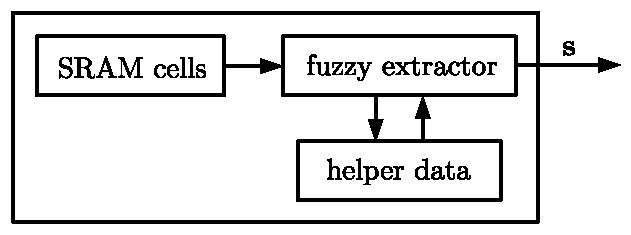
\includegraphics[width = 0.75\linewidth]{./figs/pok.pdf}
% \caption{POK uses an FE to ensure stability of the secret seed.}
% \label{fig:pok}
% \end{figure}

%We now present the details of implementing the lattice PUF, as shown in Figure \ref{fig:fpga_impl}. 
In this section, we show the hardware implementation details of lattice PUF. The entire design, except for the raw (uninitialized) SRAM cells, was synthesized, configured, and tested on a Xilinx Spartan-6 FPGA (XC6SLX45), a low-end FPGA in 45nm technology.

We adopt the homogeneous error assumption regarding the RFE design. This means all cells are assumed to have the same BER \cite{bosch2008efficient}.
The range of intrinsic BERs of the various POKs is shown to be $0.1\%$ \cite{karpinskyy20168} to $15\%$ \cite{maes2009soft}. 
We investigate four levels of raw BER: $1\%$, $5\%$, $10\%$, and $15\%$ to explore design costs in POK and RFE, and finally select $5\%$ as the raw SRAM BER in our implementation. The RFE design targets a $10^{-6}$ failure rate in reconstruction of $1280$ key bits. As described in Section \ref{sec:design}, with such a nearly-perfect rate in key reconstruction, the overall output BER of the lattice PUF can achieve the desired decryption error rate mentioned above.
We use concatenated error-correcting codes (ECC), with a repetition code as the inner code, and a shortened BCH code as the outer code.
Concatenated codes are typically more efficient than single codes in terms of code length and hardware cost \cite{bosch2008efficient}. 
As described in Section \ref{sec:design}, the RFE scheme needs only lightweight encoder implementation on the device side. 
Table \ref{table:ecc} and \ref{table:hardware_fe} show the parameters and hardware utilization of error-correcting codes configured for different BER levels respectively.
A $5\%$ raw BER requires $6.5K$ cells to construct the $1280$-bit secret $\mathbf{s}$ with a failure rate of $10^{-6}$.
The RFE encoder design requires $27$ slices. 
We adopt the SRAM-based design of \cite{aysu2015end} to implement the TRNG. The advantage is that the SRAM cells used to generate $\mathbf{s}$ can be reused for the SRAM-TRNG design. 
We adopt the 8-fold XORing of SRAM bits in \cite{aysu2015end} and therefore need $10.2K$ (i.e. $3.7K$ additional) SRAM cells. 
The 8-fold XORing logic design requires $1$ slice. 
Then, for the $5\%$ raw BER, the RFE design requires $28$ slices in total. 
%The cost of FE/RFE applies to all other strong PUF candidates (AES PUF or other controlled PUF).
%This is also cheaper than linear solver block used in the CFE-based strong PUF \cite{herder2017trapdoor,jin2017fpga} for key reconstruction, which requires $65,700$ LUTs and $16,425$ slices.

The lattice PUF (without FE) takes a total of 45 slices on Spartan-6 FPGA. The LFSR and the controller occupies most of the slices. Table \ref{table:fpga_utilization} shows the resources breakdown of each module. The LWE decryption function (LWEDec) is implemented with an 8-bit MAC and a quantization block, Figure \ref{fig:lwedec}.
RAM-based shift registers are used to implement the 256-bit LFSR. The total latency (at 33.3MHz clock) to generate a 1-bit PUF response is $47\mu$s, and the total time to generate a 100-bit PUF response is, approximately, $8\mu s + 100\times 44\mu s\approx 4.4ms$ since seed loading is only executed once. 
Table \ref{table:fpga_timing} shows latency breakdown of each step in response generation. 

We now explore the design space of the lattice PUF, starting with the resource-efficient design. We adopt the parallelization strategies proposed in Section \ref{sec: lpuf_par} and implement designs with different levels of parallelism. The latency and hardware utilization of the designs are summarized in Table \ref{table:latency_par} and \ref{table:hwslices_par}. Fig. \ref{fig:design_space_latency} and Fig. \ref{fig:design_space_hw} visualize the influence of $P_1$ and $P_2$ on latency and hardware cost. Similar to Table \ref{table:fpga_utilization}, we report the sum of slice utilization of LFSR, LWEDec and Controller modules. The maximum value of $P_2$ is $128$ due to the constraint of LFSR generator polynomial. Table entries with NA indicate the corresponding design requires more multipliers than the available DSP slices on the device. We observe that the parallelized design leads to a steady reduction in latency, at the cost of increased hardware utilization. We achieve a 148X reduction in latency in the most latency-optimized design, with a 10X increase in hardware utilization. %While both parallelization strategies demonstrate effectiveness in latency reduction, they have different efficiency in hardware utilization. 
In addition, we observe the MAC unit parallelization strategy has better hardware efficiency compared to LFSR-LWEDec datapath parallelization strategy. To achieve the same latency reduction, the design which prioritizes MAC unit parallelization requires fewer slices. For instance, to achieve the optimal $38 \mu$s latency, the design with $(P_1, P_2) = (2, 128)$ only requires $465$ slices, while the design with $(P_1, P_2) = (8, 32)$ requires $1015$ slices. This validates our optimal strategy demonstrated in Section \ref{sec: lpuf_par}. %This seems to indicate the LFSR unrolling is always a better strategy for latency optimization. However, in reality, the LFSR cannot be unrolled by unlimited times while keeping the equivalent functionality. The LFSR generator polynomial limits the maximum unrolling times. For instance, if the 256-bit LFSR takes the XOR result of $X_{255}$, $X_{253}$, $X_{250}$ and $X_{7}$ as the feedback bit, the LFSR cannot be unrolled by over 8 times with the technique presented in Section \ref{sec: lpuf_par}, since the LSB $X_{0}$ is only 8 bits away from $X_{7}$. Therefore, in practice, the optimal strategy is to first seek parallelization via LFSR unrolling, and then parallelize the LFSR-LWEDec data-path to achieve further latency optimization once the unrolling of LFSR reaches the limit.

%\begin{figure}[t!]
%\centering
%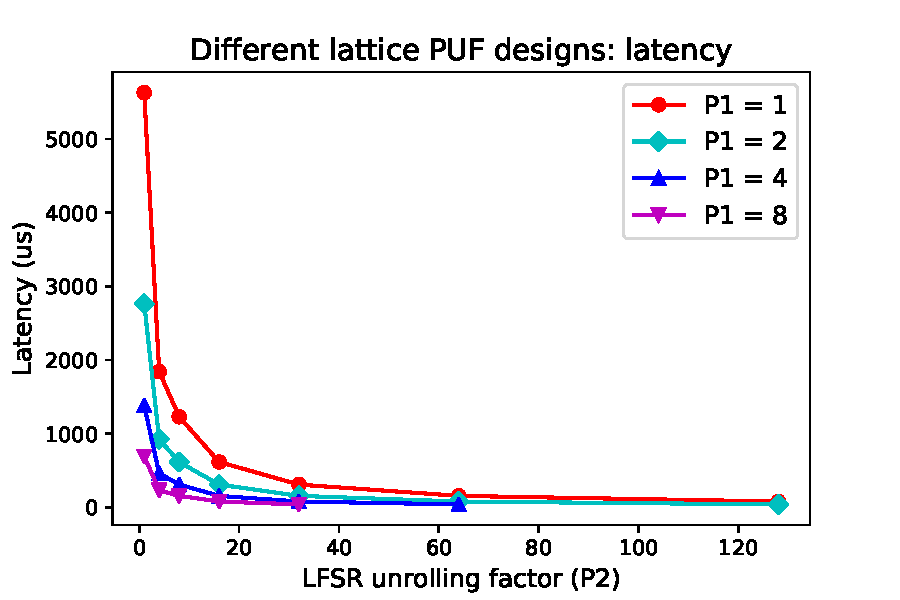
\includegraphics[width = 0.8\linewidth]{./figs/design_space_latency.pdf}
%\caption{Increasing $P_1$ and $P_2$ leads to steady reduction in latency.}
%\label{fig:design_space_latency}
%\end{figure}

%\begin{figure}[t!]
%\centering
%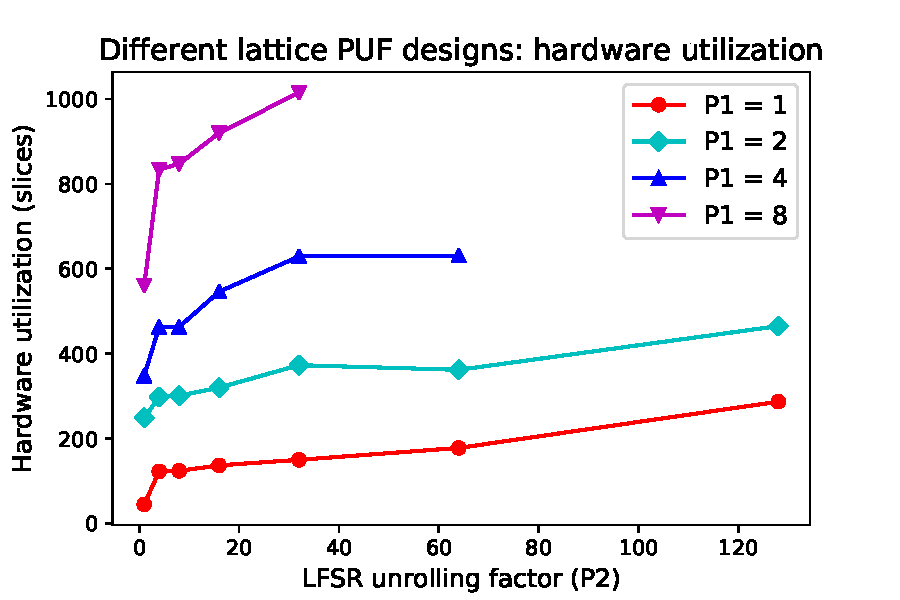
\includegraphics[width = 0.8\linewidth]{./figs/design_space_hw.pdf}
%\caption{Increasing $P_2$ is more hardware efficient than increasing $P_1$, but maximum $P_2$ is limited by the LFSR generator polynomial. The optimal strategy is to increase $P_2$ first to achieve latency goal. If $P_2$ reaches the limit and more aggressive latency reduction is required, increase $P_1$.}
%\label{fig:design_space_hw}
%\end{figure}

We finally compare the hardware utilization of the resource-efficient lattice PUF design to several published strong PUF designs \cite{bhargava2014efficient, gassend2008controlled, jin2017fpga} in Table \ref{table:hardware_puf}. 
The original proposal of the AES-based strong PUF \cite{bhargava2014efficient} is an ASIC implementation. 
Here, to estimate the AES implementation cost in FPGA, we adopt results in \cite{chu2012low}.
Note that no error correction is used in \cite{bhargava2014efficient}: it uses dark bit masking to guarantee reliability. 
Similarly, to estimate the cost of a hash function for the controlled PUF \cite{gassend2008controlled}, the FPGA implementation results of SHA-3 in \cite{kaps2011lightweight} is used.
\cite{jin2017fpga} reports the FPGA utilization result of the computational FE (CFE) based strong PUF in the number of LUTs.
We estimate the corresponding slice count using \cite{xilinx:ds190}. 
Compared to PUFs constructed with AES \cite{chu2012low} and SHA \cite{kaps2011lightweight}, our advantages in area are minor. 
However, compared to \cite{herder2017trapdoor, jin2017fpga}, which is another PUF based on LWE, and which therefore provides similar theoretical guarantees, our savings in area are significant.
%We find that the implementation cost of the lattice PUF (without FE) is cheaper than that of AES on POK, controlled PUF, and CFE-based PUF.

\begin{figure}[t!]
\centering
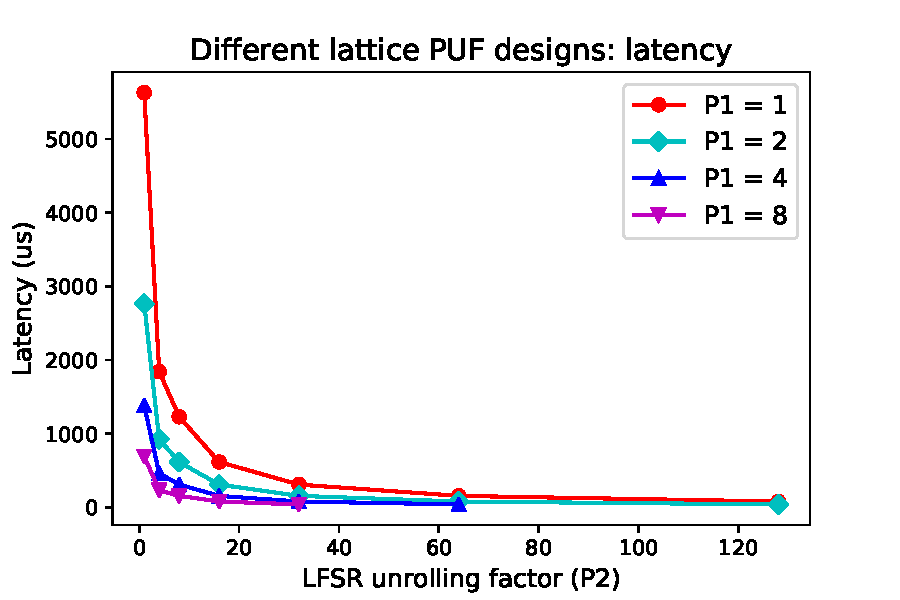
\includegraphics[width = 0.8\linewidth]{./figs/design_space_latency.pdf}
\caption{Increasing $P_1$ and $P_2$ leads to steady reduction in latency.}
\label{fig:design_space_latency}
\end{figure}

\begin{figure}[t!]
\centering
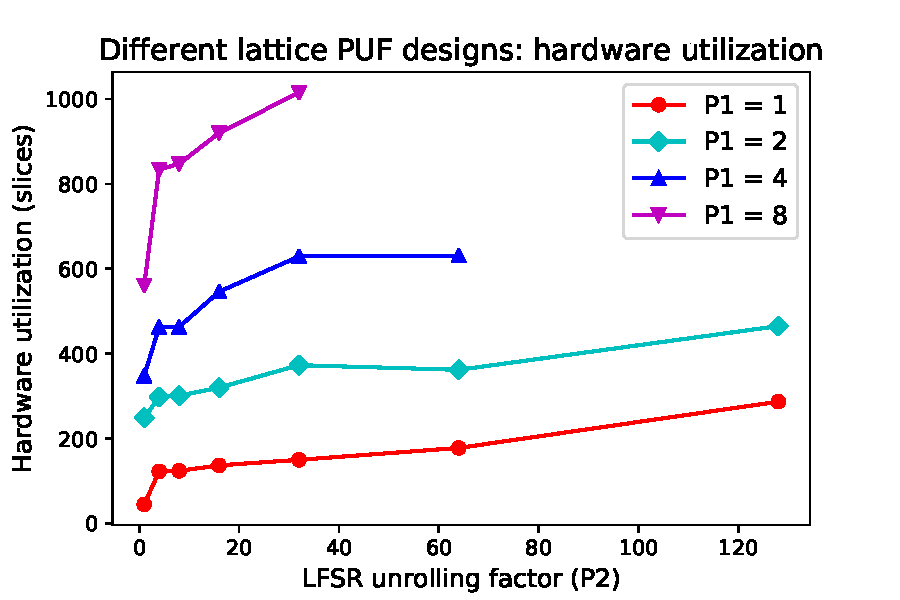
\includegraphics[width = 0.8\linewidth]{./figs/design_space_hw.pdf}
\caption{Increasing $P_2$ is more hardware efficient than increasing $P_1$, but maximum $P_2$ is limited by the LFSR generator polynomial. The optimal strategy is to increase $P_2$ first to achieve latency goal. If $P_2$ reaches the limit and more aggressive latency reduction is required, increase $P_1$.}
\label{fig:design_space_hw}
\end{figure}